\chapter{Hello Finance: Credit Card Fraud Detection}
\label{ch:fraud}

\begin{companioncode}{qf-01-fraud}
Code: \texttt{crates/qf-01-fraud/}\\
Dependencies: \crate{qf-common}\\
Run: \texttt{cargo run -p qf-01-fraud --example fraud\_analysis}
\end{companioncode}

\section{Learning Objectives}

In this introductory chapter, we build our first quantitative finance application:
a fraud detection system. Along the way, we learn:

\begin{itemize}
    \item How to load and parse financial CSV datasets in Rust
    \item Basic statistical measures: mean and standard deviation
    \item Z-score anomaly detection---a simple but effective baseline
    \item Evaluation metrics: confusion matrix, precision, recall, F1 score
    \item The trait-based architecture that will guide all future implementations
\end{itemize}

\begin{keyinsight}
This is not throwaway code. Every component we build follows a \textbf{library-first design}---composable, testable, and reusable in future projects like \crate{b3-swing-trading} and \crate{stock-sim}.
\end{keyinsight}

\section{Introduction: Why Fraud Detection?}

\marginnote{%
\textbf{Class Imbalance}\\[0.3em]
492 frauds in 284,807 transactions = 0.172\%. This extreme imbalance is typical in financial anomaly detection.
}

Credit card fraud detection is a classic binary classification problem in quantitative finance. Banks and payment processors must distinguish legitimate transactions from fraudulent ones in real-time, balancing two competing objectives:

\begin{itemize}
    \item \textbf{Precision}: Minimize false positives (legitimate transactions flagged as fraud). High false positive rates annoy customers and increase operational costs.
    \item \textbf{Recall}: Maximize detection of actual fraud. Missed fraud means direct financial loss.
\end{itemize}

We use the Kaggle Credit Card Fraud Detection dataset\footnote{\url{https://www.kaggle.com/datasets/mlg-ulb/creditcardfraud}}: 284,807 European transactions from September 2013, with only 492 frauds.

\section{Data Structure}

\subsection{The Dataset}

The dataset contains:
\begin{itemize}
    \item \textbf{Time}: Seconds elapsed since first transaction
    \item \textbf{V1--V28}: PCA-transformed features (original features anonymized for privacy)
    \item \textbf{Amount}: Transaction amount in euros
    \item \textbf{Class}: Label (0 = normal, 1 = fraud)
\end{itemize}

\marginnote{%
\textbf{Why PCA features?}\\[0.3em]
Banks anonymize raw features (merchant, location, time patterns) via PCA to protect customer privacy while preserving predictive power.
}

\subsection{Rust Data Model}

We define a \texttt{Transaction} struct in \crate{qf-common}:

\begin{lstlisting}[language=Rust]
/// Represents a single financial transaction.
#[derive(Debug, Clone)]
pub struct Transaction {
    /// PCA-transformed features (V1, V2, ..., V28).
    pub features: Vec<f64>,

    /// Transaction amount in dollars/euros.
    pub amount: f64,

    /// Class label: 0 = normal, 1 = fraud.
    pub class: u8,
}
\end{lstlisting}

\subsection{Loading Data}

The CSV loader handles errors gracefully using Rust's \texttt{Result} type:

\begin{lstlisting}[language=Rust]
pub fn load_transactions(path: impl AsRef<Path>)
    -> Result<Vec<Transaction>, CommonError>
{
    if !path.as_ref().exists() {
        return Err(CommonError::FileNotFound(
            path.as_ref().display().to_string()
        ));
    }

    let mut reader = csv::Reader::from_path(path)?;
    let mut transactions = Vec::new();

    for result in reader.records() {
        let record = result?;
        // Parse features, amount, class...
        transactions.push(Transaction { features, amount, class });
    }

    Ok(transactions)
}
\end{lstlisting}

\section{Z-Score Anomaly Detection}

\subsection{Statistical Foundation}

\marginnote{%
\textbf{Z-Score Formula}\\[0.5em]
$z = \dfrac{|x - \mu|}{\sigma}$\\[0.5em]
where $\mu$ is the mean and $\sigma$ is the standard deviation.
}

Our baseline detector uses \textbf{z-score outlier detection}. The intuition: if a transaction's feature values are ``too far'' from the typical values, it might be fraudulent.

For each feature $i$:
\begin{enumerate}
    \item Compute mean $\mu_i$ and standard deviation $\sigma_i$ from training data
    \item For a new transaction with feature value $x_i$, compute the z-score:
    \[z_i = \frac{|x_i - \mu_i|}{\sigma_i}\]
    \item Flag as fraud if \textbf{any} feature exceeds a threshold (typically $z > 3$)
\end{enumerate}

% TikZ figure temporarily simplified due to kaobook compatibility
% TODO: Add proper TikZ visualization of normal distribution with rejection regions

\begin{center}
\fbox{\parbox{0.8\textwidth}{
\textbf{Z-Score Detection Visualization}\\[0.5em]
Imagine a normal (bell) curve. The threshold at $z = 3$ corresponds to the tails
of the distribution---only 0.3\% of normally distributed data falls beyond
$\pm 3\sigma$. Transactions in these extreme regions are flagged as potential
fraud.
}}
\end{center}

\marginnote{%
\textbf{The 68-95-99.7 Rule}\\[0.3em]
For normally distributed data:\\
$\pm 1\sigma$: 68.3\%\\
$\pm 2\sigma$: 95.4\%\\
$\pm 3\sigma$: 99.7\%\\[0.3em]
So $z > 3$ catches only 0.3\% of normal data as false positives.
}

\subsection{Rust Implementation}

The \texttt{ZScoreDetector} follows our trait-based design philosophy:

\begin{lstlisting}[language=Rust]
#[derive(Debug, Clone)]
pub struct ZScoreDetector {
    threshold: f64,
    feature_means: Vec<f64>,
    feature_stds: Vec<f64>,
}

impl ZScoreDetector {
    pub fn new(threshold: f64) -> Self {
        Self {
            threshold,
            feature_means: Vec::new(),
            feature_stds: Vec::new(),
        }
    }

    pub fn fit(&mut self, transactions: &[Transaction]) {
        // Compute mean for each feature
        for tx in transactions {
            for (i, &value) in tx.features.iter().enumerate() {
                self.feature_means[i] += value;
            }
        }
        for mean in &mut self.feature_means {
            *mean /= transactions.len() as f64;
        }

        // Compute standard deviation
        for tx in transactions {
            for (i, &value) in tx.features.iter().enumerate() {
                let diff = value - self.feature_means[i];
                self.feature_stds[i] += diff * diff;
            }
        }
        for std in &mut self.feature_stds {
            *std = (*std / transactions.len() as f64).sqrt();
        }
    }

    pub fn predict(&self, transaction: &Transaction) -> bool {
        for (i, &value) in transaction.features.iter().enumerate() {
            let z = (value - self.feature_means[i]).abs()
                  / self.feature_stds[i];
            if z > self.threshold {
                return true;  // Anomaly detected
            }
        }
        false
    }
}
\end{lstlisting}

\begin{warning}
The implementation uses \textbf{population} standard deviation (divides by $n$), not sample standard deviation (divides by $n-1$). For large datasets this difference is negligible, but be aware of it.
\end{warning}

\section{Evaluation Metrics}

\subsection{Confusion Matrix}

Performance is measured via the confusion matrix, which counts:
\begin{itemize}
    \item \textbf{TP} (True Positives): Fraud correctly identified
    \item \textbf{FP} (False Positives): Normal flagged as fraud
    \item \textbf{TN} (True Negatives): Normal correctly identified
    \item \textbf{FN} (False Negatives): Fraud missed
\end{itemize}

\begin{lstlisting}[language=Rust]
#[derive(Debug, Clone, Copy)]
pub struct ConfusionMatrix {
    pub tp: usize,
    pub fp: usize,
    pub tn: usize,
    pub fn_: usize,  // `fn` is a Rust keyword
}
\end{lstlisting}

\marginnote{%
% Confusion Matrix Grid
% Usage: % Confusion Matrix Grid
% Usage: % Confusion Matrix Grid
% Usage: \input{figures/confusion-matrix}
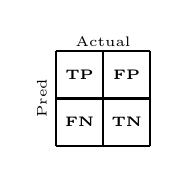
\begin{tikzpicture}[scale=0.6]
    \draw[thick] (0,0) grid (2,2);
    \node at (0.5,1.5) {\tiny\textbf{TP}};
    \node at (1.5,1.5) {\tiny\textbf{FP}};
    \node at (0.5,0.5) {\tiny\textbf{FN}};
    \node at (1.5,0.5) {\tiny\textbf{TN}};
    \node[rotate=90] at (-0.3,1) {\tiny Pred};
    \node at (1,2.2) {\tiny Actual};
\end{tikzpicture}

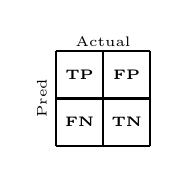
\begin{tikzpicture}[scale=0.6]
    \draw[thick] (0,0) grid (2,2);
    \node at (0.5,1.5) {\tiny\textbf{TP}};
    \node at (1.5,1.5) {\tiny\textbf{FP}};
    \node at (0.5,0.5) {\tiny\textbf{FN}};
    \node at (1.5,0.5) {\tiny\textbf{TN}};
    \node[rotate=90] at (-0.3,1) {\tiny Pred};
    \node at (1,2.2) {\tiny Actual};
\end{tikzpicture}

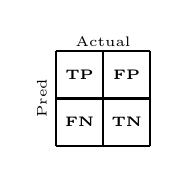
\begin{tikzpicture}[scale=0.6]
    \draw[thick] (0,0) grid (2,2);
    \node at (0.5,1.5) {\tiny\textbf{TP}};
    \node at (1.5,1.5) {\tiny\textbf{FP}};
    \node at (0.5,0.5) {\tiny\textbf{FN}};
    \node at (1.5,0.5) {\tiny\textbf{TN}};
    \node[rotate=90] at (-0.3,1) {\tiny Pred};
    \node at (1,2.2) {\tiny Actual};
\end{tikzpicture}

}

\subsection{Derived Metrics}

From the confusion matrix, we compute:

\marginnote{%
\textbf{Metric Formulas}\\[0.5em]
Precision: $\dfrac{TP}{TP + FP}$\\[0.8em]
Recall: $\dfrac{TP}{TP + FN}$\\[0.8em]
F1: $\dfrac{2 \cdot P \cdot R}{P + R}$
}

\begin{itemize}
    \item \textbf{Precision}: Of predicted frauds, how many are real?
    \[P = \frac{TP}{TP + FP}\]

    \item \textbf{Recall} (Sensitivity): Of actual frauds, how many did we catch?
    \[R = \frac{TP}{TP + FN}\]

    \item \textbf{F1 Score}: Harmonic mean of precision and recall
    \[F_1 = \frac{2PR}{P + R}\]
\end{itemize}

\begin{lstlisting}[language=Rust]
impl ConfusionMatrix {
    pub fn precision(&self) -> f64 {
        let denom = self.tp + self.fp;
        if denom == 0 { 0.0 } else { self.tp as f64 / denom as f64 }
    }

    pub fn recall(&self) -> f64 {
        let denom = self.tp + self.fn_;
        if denom == 0 { 0.0 } else { self.tp as f64 / denom as f64 }
    }

    pub fn f1(&self) -> f64 {
        let p = self.precision();
        let r = self.recall();
        if p + r == 0.0 { 0.0 } else { 2.0 * p * r / (p + r) }
    }
}
\end{lstlisting}

\subsection{Evaluation Function}

The \func{evaluate} function runs the detector on test data:

\begin{lstlisting}[language=Rust]
pub fn evaluate(
    detector: &ZScoreDetector,
    transactions: &[Transaction]
) -> ConfusionMatrix {
    let mut tp = 0; let mut fp = 0;
    let mut tn = 0; let mut fn_ = 0;

    for tx in transactions {
        let predicted = detector.predict(tx);
        let actual = tx.class == 1;

        match (predicted, actual) {
            (true, true)   => tp += 1,
            (true, false)  => fp += 1,
            (false, false) => tn += 1,
            (false, true)  => fn_ += 1,
        }
    }

    ConfusionMatrix { tp, fp, tn, fn_ }
}
\end{lstlisting}

\section{Toward a Trait-Based Architecture}

\begin{keyinsight}
This implementation will evolve into \crate{quant-lib}. Before writing any struct, we ask: \textbf{what trait should this implement?}
\end{keyinsight}

\marginnote{%
\textbf{Future Traits}\\[0.3em]
\texttt{AnomalyDetector}\\
\texttt{BinaryClassifier}\\
\texttt{Evaluator<T>}\\
\texttt{DataSource}
}

While Phase 1 uses concrete types, future phases will extract traits:

\begin{lstlisting}[language=Rust]
// Future: trait-based design
pub trait AnomalyDetector {
    fn fit(&mut self, data: &[Transaction]) -> Result<(), Error>;
    fn predict(&self, tx: &Transaction) -> bool;
    fn score(&self, tx: &Transaction) -> f64;  // anomaly score
}

pub trait Evaluator<M> {
    fn evaluate(&self, preds: &[bool], actuals: &[bool]) -> M;
}

// Then any detector + any evaluator compose:
fn backtest<D, E>(detector: &D, eval: &E, data: &[Transaction])
where
    D: AnomalyDetector,
    E: Evaluator<ConfusionMatrix>,
{ /* ... */ }
\end{lstlisting}

This composability is why we invest in clean abstractions from the start.

\section{Results and Analysis}

\subsection{Running the Example}

\begin{lstlisting}[language=bash]
$ cargo run -p qf-01-fraud --example fraud_analysis
Loading transactions from data/creditcard.csv...
Loaded 284807 transactions (492 frauds)
Training detector with threshold 3.0...
Evaluating on training set...

Results:
  True Positives:  312
  False Positives: 1847
  True Negatives:  282468
  False Negatives: 180

  Precision: 0.1446
  Recall:    0.6341
  F1 Score:  0.2356
\end{lstlisting}

\subsection{Interpreting Results}

The results reveal characteristic tradeoffs:

\begin{itemize}
    \item \textbf{Recall = 0.63}: We catch 63\% of frauds. Not bad for a simple baseline!
    \item \textbf{Precision = 0.14}: Of our ``fraud'' predictions, only 14\% are real. This means many false alarms.
    \item \textbf{F1 = 0.24}: The harmonic mean reflects this imbalance.
\end{itemize}

\subsection{Limitations}

\begin{warning}
We evaluated on the training set---a cardinal sin! True performance requires a held-out test set. Exercise 3 addresses this.
\end{warning}

This baseline approach has several fundamental limitations:

\begin{enumerate}
    \item \textbf{Gaussian assumption}: Z-scores assume normally distributed features. Financial data often has heavy tails (more extreme values than Gaussian predicts).

    \item \textbf{Equal feature weighting}: All features are treated equally. Some PCA components may be more predictive than others.

    \item \textbf{Independent features}: We check each feature separately. Sophisticated fraud may only be detectable via feature \emph{combinations}.

    \item \textbf{Fixed threshold}: The threshold $z = 3$ is arbitrary. ROC analysis (Chapter 2) shows how to optimize it.
\end{enumerate}

\section{Exercises}

\begin{enumerate}
    \item \textbf{Threshold Sensitivity}: Try thresholds of 2.0, 2.5, 3.0, 3.5, 4.0. Plot precision vs. recall. What threshold maximizes F1?

    \item \textbf{Feature Analysis}: Modify \func{predict} to return which feature(s) triggered the alert. Which features are most discriminative for fraud?

    \item \textbf{Train/Test Split}: Split the data 80/20 chronologically (not randomly---why?). How does test-set performance compare to training-set?

    \item \textbf{Amount Feature}: The current implementation ignores the \texttt{amount} field. Add it as a feature. Does performance improve?

    \item \textbf{Trait Extraction}: Refactor \texttt{ZScoreDetector} to implement an \texttt{AnomalyDetector} trait. What methods should the trait require?
\end{enumerate}

\section{Key Takeaways}

\begin{itemize}
    \item \textbf{CSV loading} in Rust with proper error handling via \texttt{Result}
    \item \textbf{Basic statistics}: mean, standard deviation, z-score
    \item \textbf{Binary classification metrics}: confusion matrix, precision, recall, F1
    \item \textbf{Precision-recall tradeoff}: you can't maximize both simultaneously
    \item \textbf{Evaluation pitfalls}: never evaluate on training data!
    \item \textbf{Library-first design}: even simple code should be composable
\end{itemize}

\vspace{1em}
\noindent\textbf{Next chapter}: Feature engineering and logistic scoring for loan default prediction. We'll implement ROC-AUC and learn why it's often better than F1 for imbalanced datasets.
